\section{Document Certificates \& Binding Encryptions}
Before, all communication sent ``\textbf{over the wire}'' (from device to device),
was sent ``\textbf{in the clear}'' (unencrypted). This means that anyone could 
view data sent between devices in plain text. This is a problem when setting up 
infrastructure such as banking, e-commerce, or any other service that requires
sensitive information to be sent over the internet.

\begin{Def}[Integrity \& Authenticity]

    \textbf{Integrity} is the assurance that data has not been altered in transit.\\
    \textbf{Authenticity} is the assurance that the data is coming from the correct source.
\end{Def}
\begin{Def}[Transport Layer Security (TLS)]

    TLS is a protocol providing end-to-end encryption of data. It authenticates
    the server via \textbf{TLS certificates} to ensure the client is connecting to 
    the correct host. It also ensures integrity of the data.

    The Engineering Task Force (IETF) published the first version of TLS in 1999. As of 
    today the most recent version is TLS 1.3. (2018).
    \hfill \cite{cloudflare_tls}
\end{Def}

\begin{Def}[Secure Sockets Layer (SSL) [Deprecated]]

    SSL is the predecessor to TLS. It was developed by Netscape in the 1990s. 
    SSL 3.0 was released in 1996. SSL 3.0 was found to be insecure and was replaced
    by TLS 1.0 in 1999.
    \hfill \cite{cloudflare_tls}
\end{Def}

\begin{Def}[Certificate Authority (CA)]

    A CA is a third-party entity that issues digital certificates. Often called \textbf{SSL certificates} or TLS certificates.
    The protocol supports both SSL and TLS. Despite SSL's deprecation the name stuck due branding issues.
    Browsers and Operating systems have a list of trusted CAs called the \textbf{root store}.
    A full list of Microsoft's trusted CAs can be found here:\\ \href{https://ccadb.my.salesforce-sites.com/microsoft/IncludedCACertificateReportForMSFT}{https://ccadb.my.salesforce-sites.com/microsoft/...}
    \hfill \cite{kinsta_tls_ssl}
\end{Def}

\newpage 

\begin{Def}[Encryption]

    \textbf{Encryption} is the process of converting plaintext into ciphertext (indiscernible text).\\
    \textbf{Decryption} is the process of converting ciphertext back into plaintext.

\end{Def}
\begin{Def}[Symmetric \& Asymmetric Encryption]
    
    \textbf{Key}: is a seed/piece of information used to encrypt or decrypt data.\\
    \textbf{Symmetric Encryption}: uses the same key for both encryption and decryption.\\
    \textbf{Asymmetric Encryption}: uses a public key for encryption and a private key for decryption.\\
    ${}$ \hfill \cite{adetunji_symmetric_asymmetric_encryption}
\end{Def}

\vspace{-1em}
\begin{figure}[h!]
    \centering
    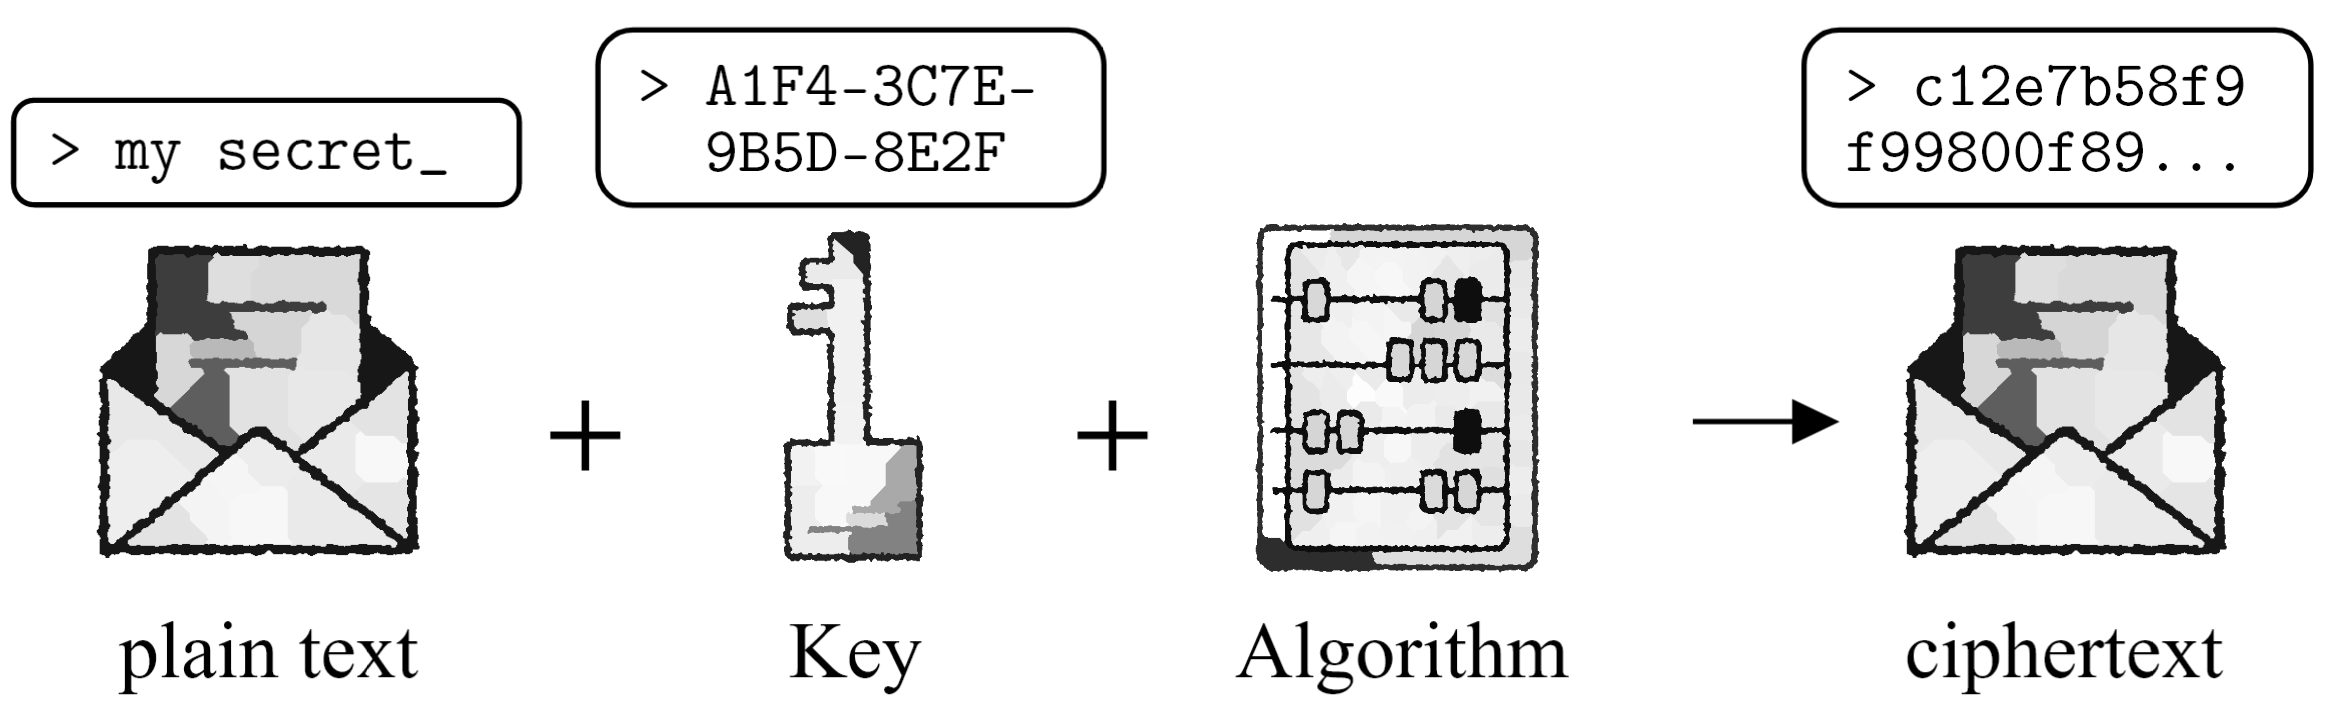
\includegraphics[width=1\textwidth]{Sections/sec/encrypt.png}
    \caption{High-level depiction of encryption.}
    \label{fig:encryption}
\end{figure}

\noindent
Encryption takes a key, data, and an algorithm to produce ciphertext.
Decryption takes the same key, ciphertext, and algorithm to produce the original data.

\vspace{1em}
\begin{Def}[Hashing]
    \textbf{Hashing} is the process of converting data into a fixed-length string of characters.
    Hashing is a one-way function, meaning it cannot be reversed (theoretically). In practice, 
    it is computationally infeasible to reverse a hash without brute force (trying all possible inputs) 
    or exploiting weaknesses in the hashing algorithm. Some hash algorithms use the text itself 
    as input, while others may incorporate a separate key (e.g., HMAC). \hfill \cite{codecademy_hashing}
\end{Def}

\begin{Def}[Hypertext Transfer Protocol Secure (HTTPS)]

    A version of HTTP that uses TLS to encrypt data. \hfill \cite{cloudflare_http_not_secure}
\end{Def}


\newpage 
\begin{Def}[SSL/TLS Certificate Specifications]

    \begin{itemize}
        \item \textbf{Common Name (CN)}: The domain name the certificate is issued for.
        \item \textbf{Subject Alternative Name (SAN)}: Additional domain names or subdomains covered by the certificate.
        \item \textbf{Key Length}: A minimum of 2048 bits, ensuring strong encryption.
        \item \textbf{Hashing Algorithm}: Typically SHA-256 for secure data integrity.
        \item \textbf{Valid From/To}: The validity period, usually up to 397 days.
        \item \textbf{Issuer}: The trusted Certificate Authority (CA) that issued the certificate.
        \item \textbf{Extended Key Usage}: Specifies purposes like server authentication or client authentication.
    \end{itemize}
    \hfill \cite{kinsta_tls_ssl}
\end{Def}

\begin{figure}[h!]
    \centering
    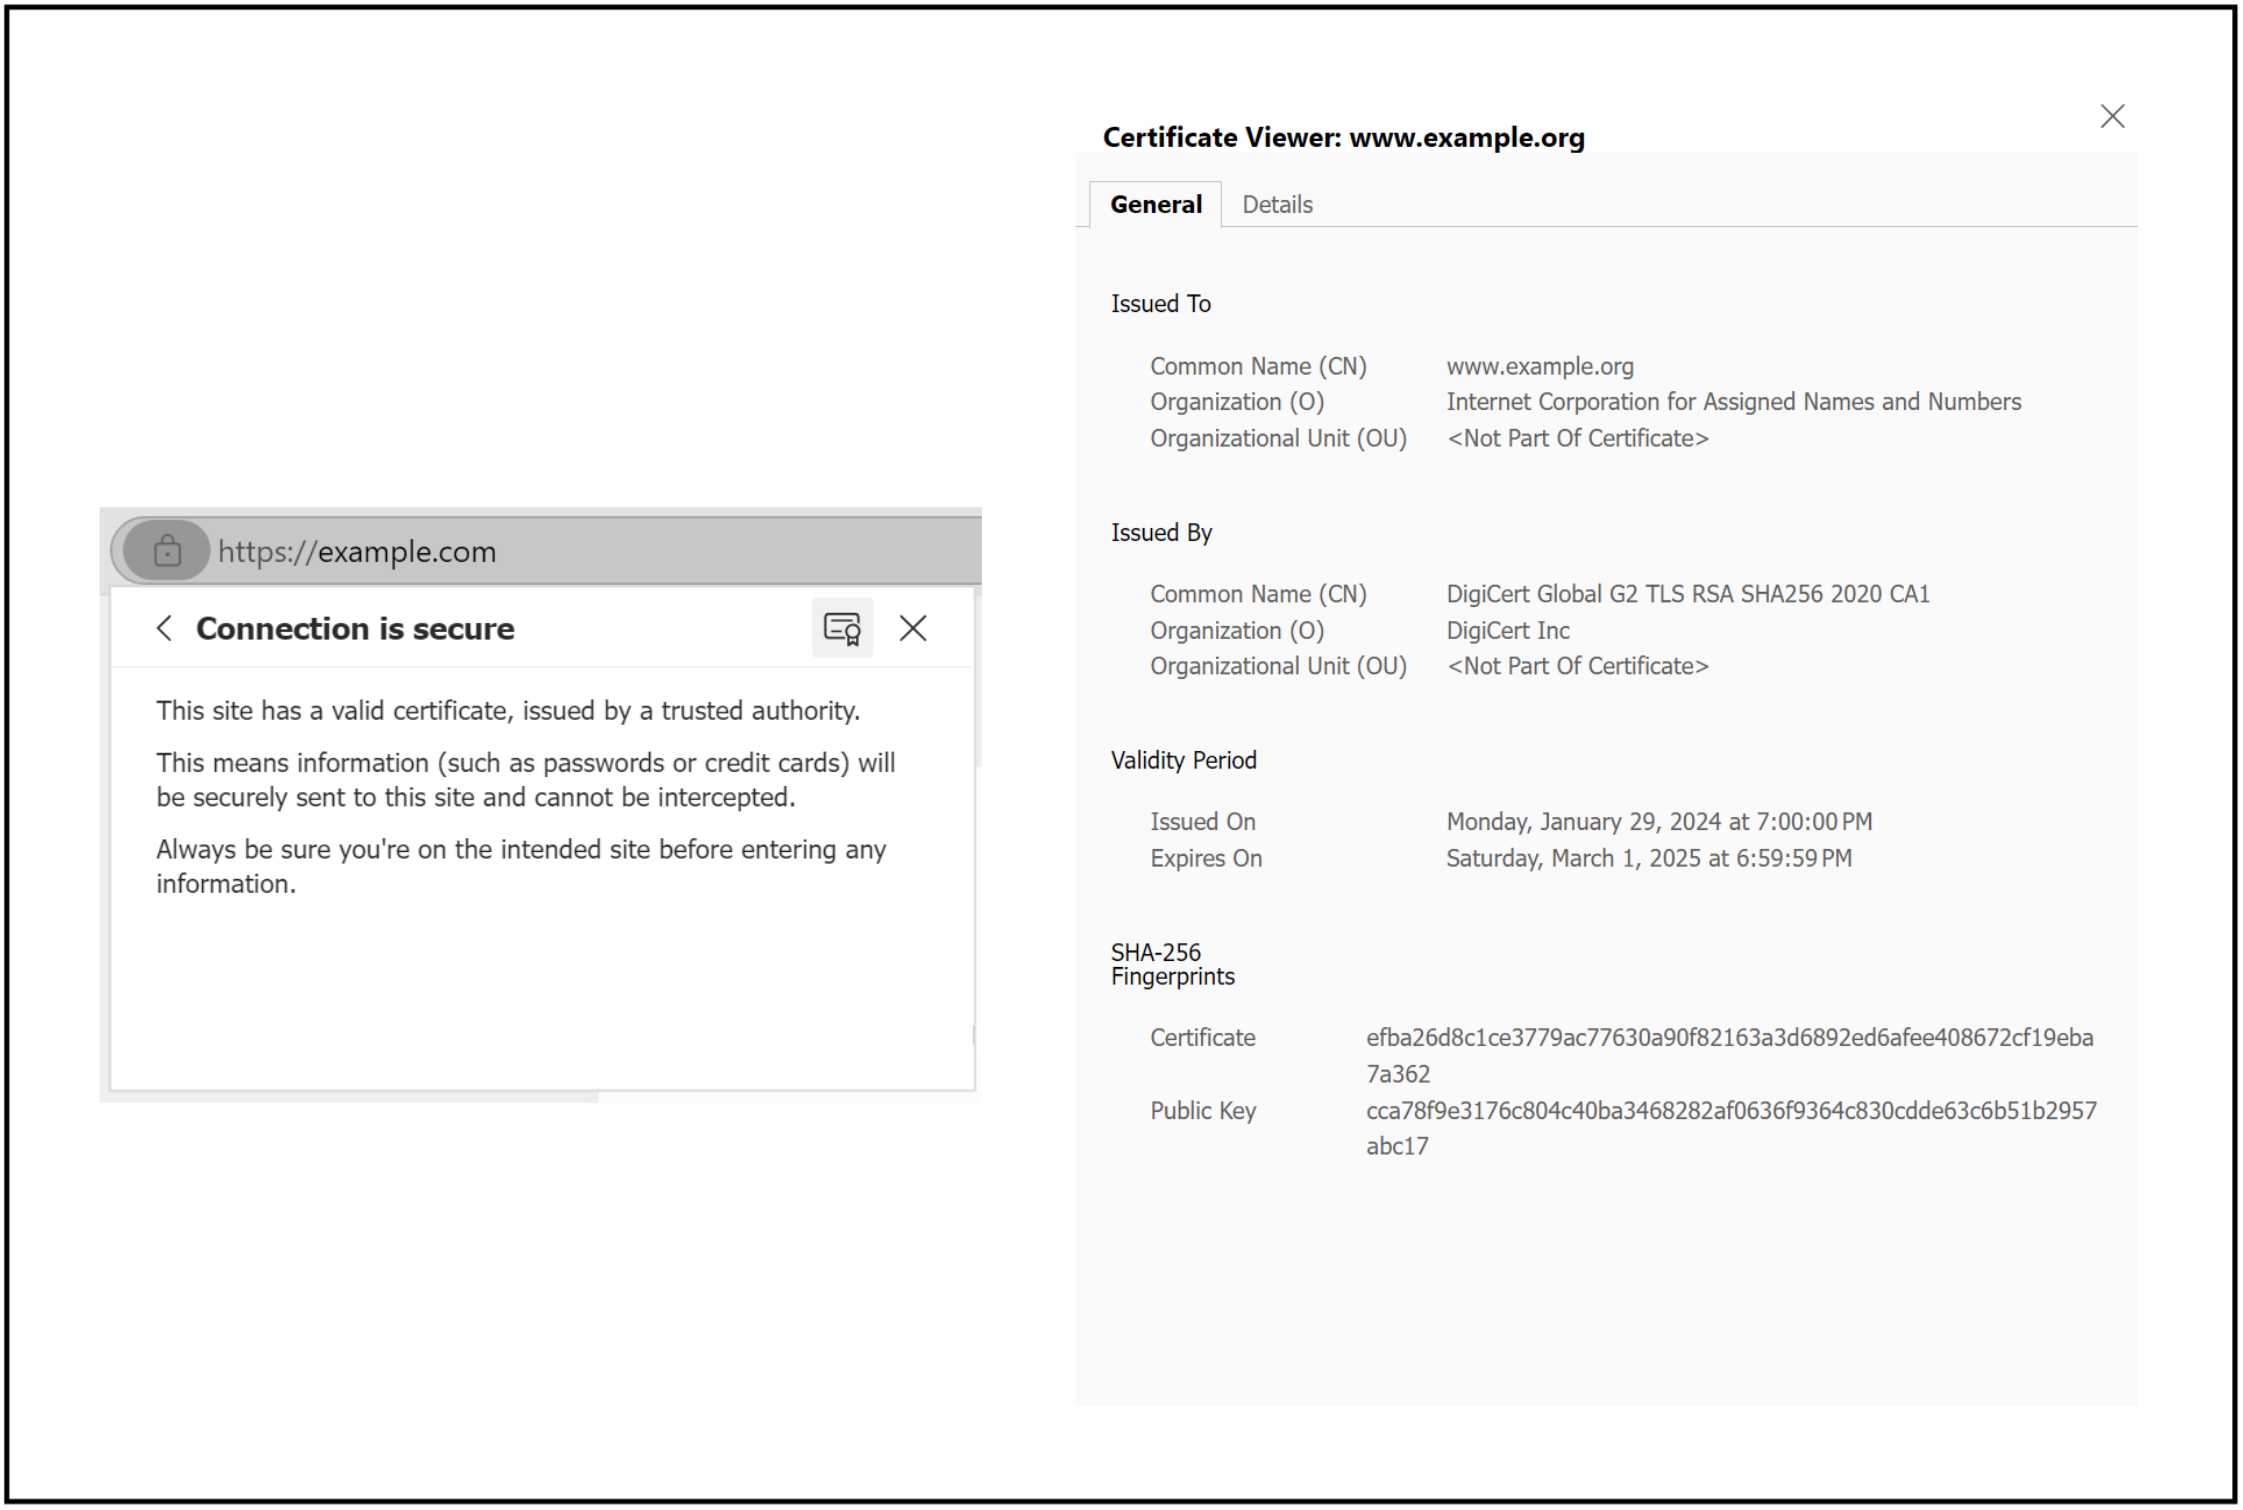
\includegraphics[width=1\textwidth]{Sections/sec/cert.png}
    \caption{SSL certificate obtained through the Edge browser on example.com}
    \label{fig:cert}
\end{figure}

\newpage 

\begin{Def}[Public Key Infrastructure (PKI)]

    PKI is a system for managing digital certificates. It includes the creation, distribution, and revocation of certificates.
    PKI is used to secure data transmission over the internet such as secure email, VPNs, and other services.
    \hfill \cite{okta_pki}
\end{Def}

\begin{Def}[Digtial \& Authority Certificates]

    \textbf{Digital Certificate}: An electronic document binding and proving ownership of a public key.\\
    \textbf{Authority Certificate}: or \textbf{Root Certificate} issued by a CA, signs other certificates.
    it is \textbf{self-signed} and is the top of the certificate chain.
    
    This establishes layers of trust and distance between the root certificate and the end-user certificates.
    If the root certificate is compromised, all certificates through the chain are compromised.
    \hfill \cite{yitzhak_digital_certificates}
\end{Def}

\begin{Def}[Digital Signatures]
    
    To verify a source, a \textbf{digital signature} is used. 
    \begin{itemize}
        \item \textbf{Key Generation}: A private and public key pair is generated beforehand.
        \item \textbf{Hashing}: A cryptographic hash of the data is created (e.g., SHA-256).
        \item \textbf{Encryption}: The private key encrypts the hash, creating the digital signature through an algorithm (e.g., RSA).
        \item \textbf{Verification}: The recipient decrypts the signature with the public key and compares the result to their own hash of the data. \hfill \cite{cisa_digital_signatures}
    \end{itemize}
\end{Def}

\begin{Def}[Certificate Signing Request (CSR)]

    To obtain a digital certificate, a client generates a CSR, which involves the following steps:
    \begin{enumerate}
        \item \textbf{Generate Key Pair}: Create a private key (kept secret) and a public key (shared).
        \item \textbf{Produce CSR Data}: Include identifying information (e.g., Organization (O), Common Name (CN)), the public key, and other details in a standardized format such as X.509.
        \item \textbf{Sign the CSR}: Hash the CSR data and sign it using the private key to prove ownership.
        \item \textbf{Submit and Issue Certificate}: Submit the CSR to a CA, which validates the signature, signs the certificate with its own private key, and issues the certificate.
        \hfill \cite{rfc2986}
    \end{enumerate}
\end{Def}


\begin{figure}[h!]
    \centering
    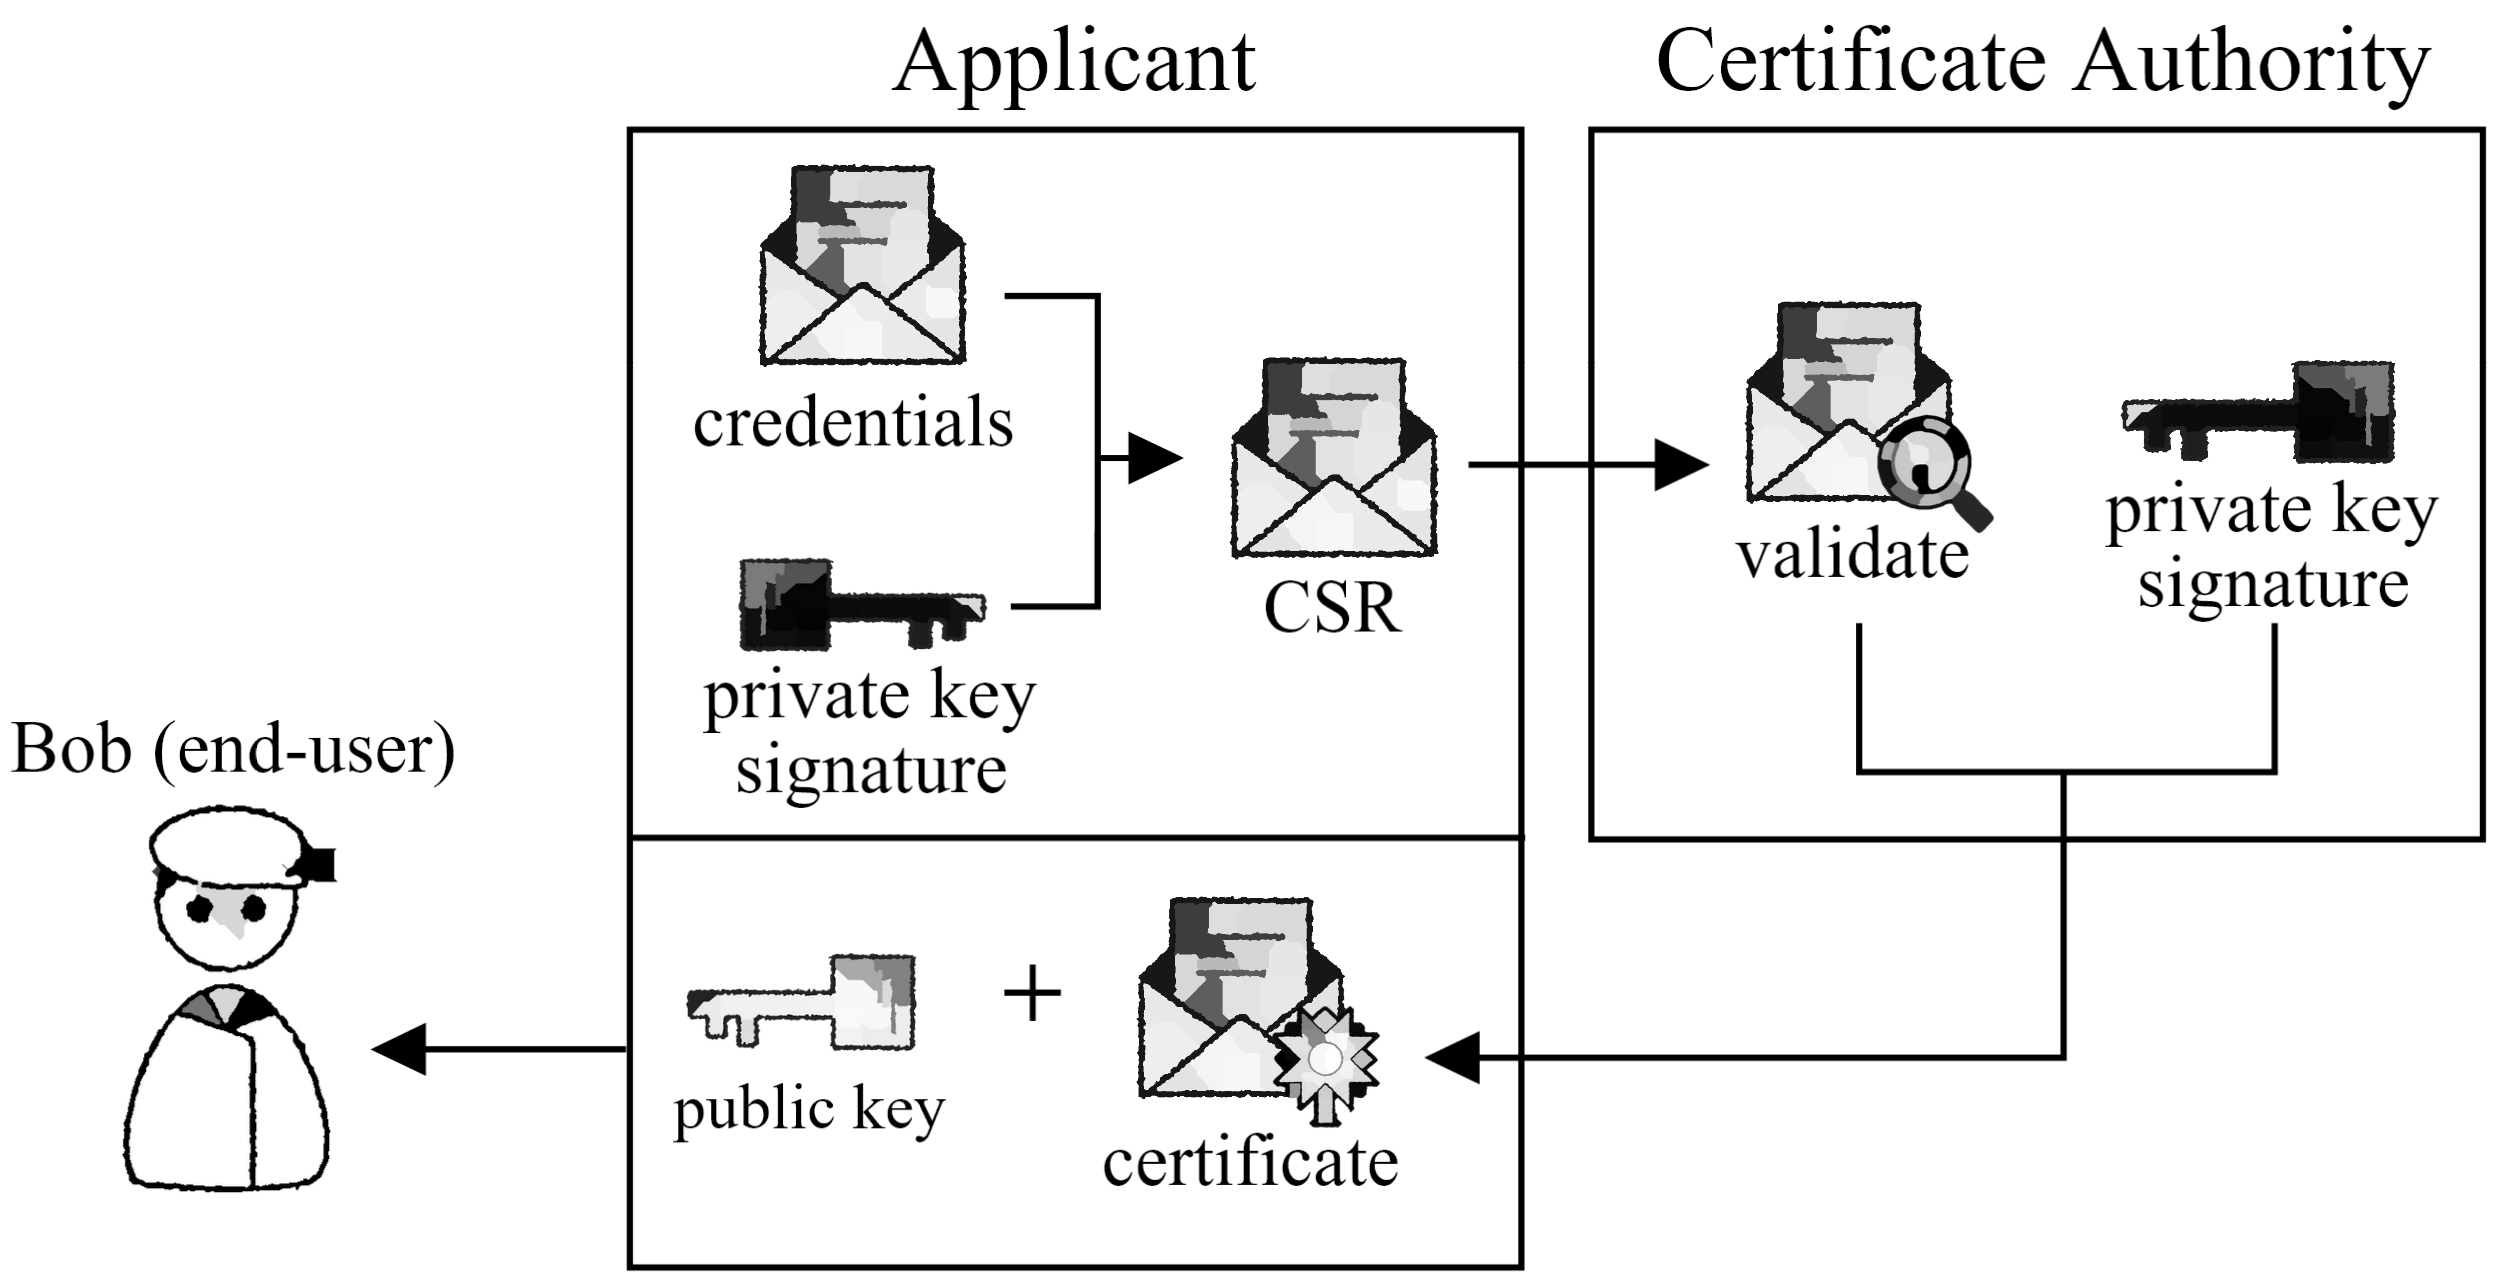
\includegraphics[width=1\textwidth]{Sections/sec/csr.png}
    \caption{Example of a Certificate Signing Request (CSR)}
    \label{fig:csr}
\end{figure}

\begin{Def}[Certificate Revocation List (CRL)]

    A CRL is a list of certificates that have been revoked by the CA before their expiration date.
    This is used to prevent the use of compromised certificates.
    \hfill \cite{rfc5280}
\end{Def}

\begin{Def}[Chain of Trust]

    A \textbf{Chain of Trust} is a hierarchical sequence of certificates used in PKI to establish trust between entities. It consists of:
    \begin{itemize}
        \item \textbf{Root Certificates}: Self-signed certificates at the top of the trust chain, trusted directly by operating systems and browsers.
        \item \textbf{Intermediate Certificates}: Issued by the root CA to delegate trust, adding a layer of security by isolating the root CA from direct interactions.
        \item \textbf{End-Entity Certificates}: Issued to users, servers, or devices to authenticate their identity and enable secure communications.
    \end{itemize}
    Each certificate is digitally signed by the private key of the certificate authority above it in the chain, with the root certificate serving as the ultimate trust anchor.
    Certified issuers are preferred over self-signed certificates because they undergo rigorous external validation, creating a verifiable path of trust. \hfill \cite{rfc5280}
\end{Def}

\newpage 

\begin{figure}[h!]
    \centering
    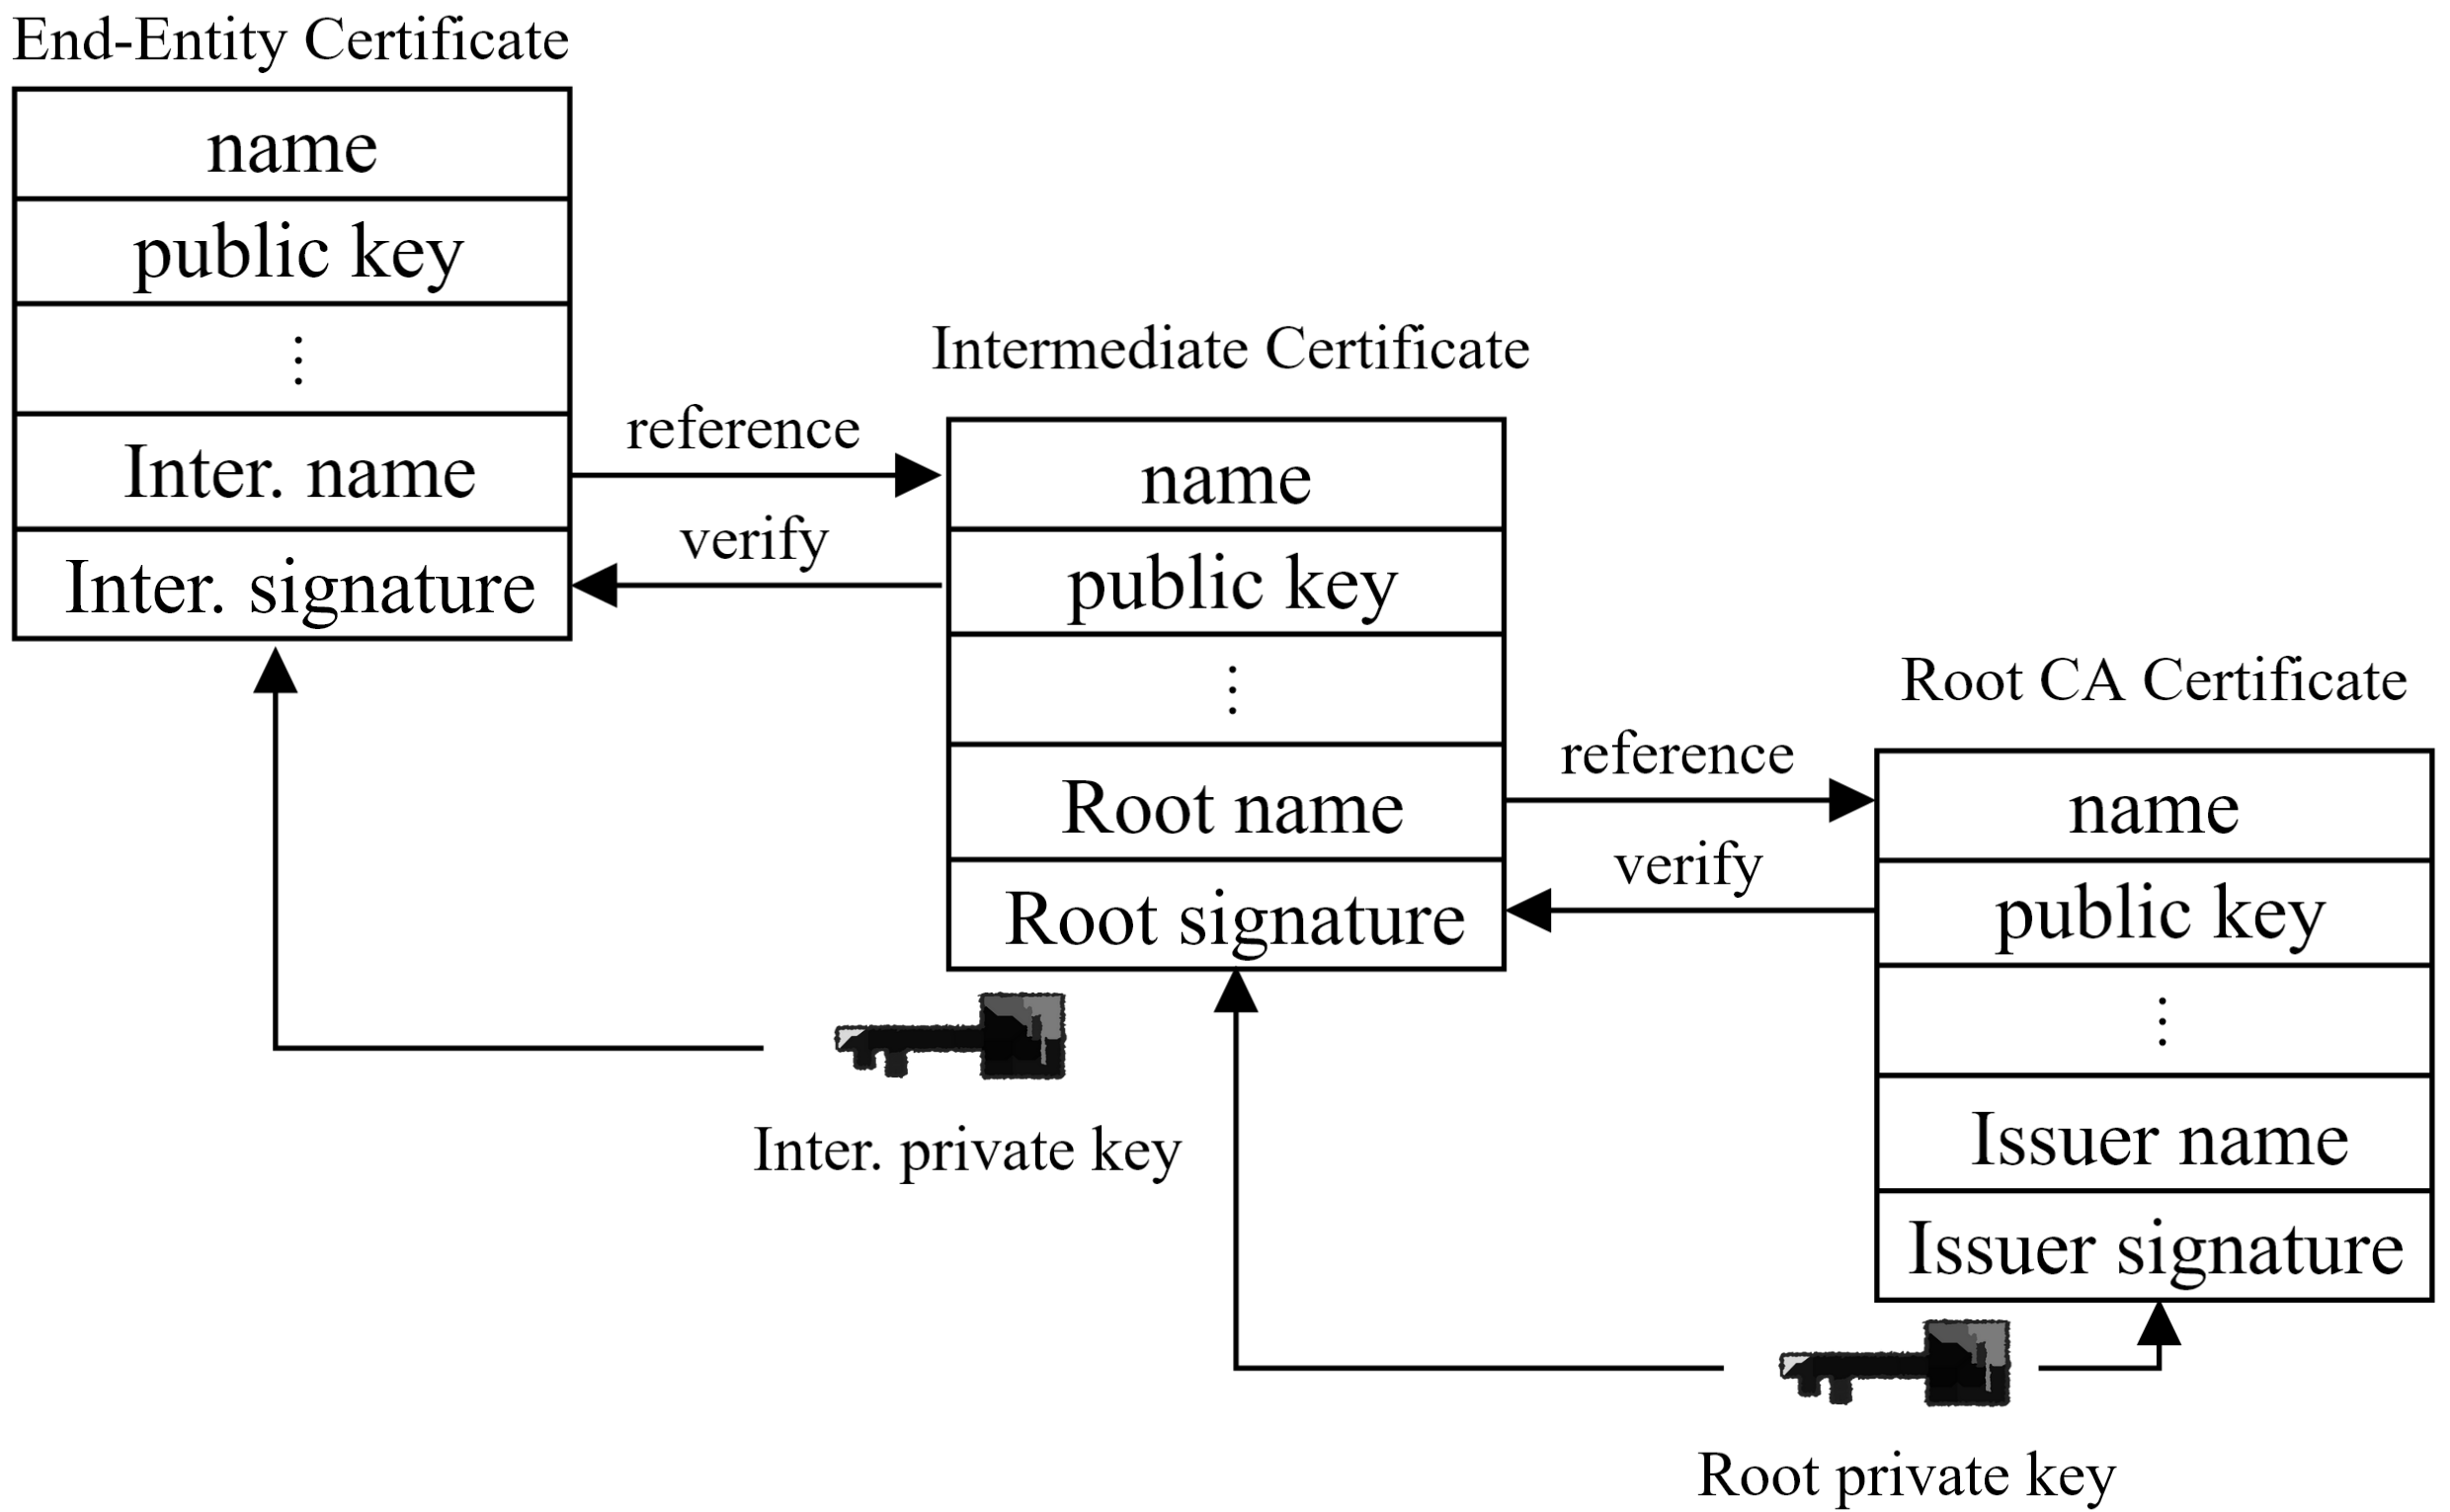
\includegraphics[width=1\textwidth]{Sections/sec/chain.png}
    \caption{A Chain of Trust from the Root Certificate to the End-Entity Certificate.}
    \label{fig:chain}
\end{figure}

\begin{Def}[Root Certificate Authority (CA) Signing Ceremonies]

    A \textbf{Root Certificate Authority (CA) Signing Ceremony} is a highly secure process in which a Root CA's private key is used to sign subordinate certificates, establishing trust within a Public Key Infrastructure (PKI). Key characteristics include:

    \begin{itemize}
        \item \textbf{Rigorous Security}: Conducted in offline, access-controlled environments with multiple layers of physical and procedural security. Entry requires the presence of multiple trusted individuals simultaneously.
        \item \textbf{Defined Roles}: Roles such as Crypto Officers, Witnesses, and Administrators are assigned to ensure transparency and accountability.
        \item \textbf{Global Trust Anchors}: Managed by organizations like ICANN for DNSSEC, these ceremonies protect the integrity of critical internet infrastructure.
        \item \textbf{Independent Operations}: Root CAs are typically independent from government oversight, though some, like the
        U.S. Department of Defense, manage government-affiliated Root CAs. 
    \end{itemize}
    Learn More: \href{https://www.cloudflare.com/learning/dns/dnssec/root-signing-ceremony/#:~:text=That%E2%80%99s%20the%20purpose%20of%20the%20Root%20Signing%20Ceremony%E2%80%94a,literally%20the%20key%20to%20the%20entire%20DNSSEC-protected%20Internet.}{https://cloudflare.com/learning/dns/dnssec/root-signing-ceremony/} \hfill \cite{cloudflare_root_signing}
\end{Def}

\newpage 

\begin{Def}[DNS over HTTPS (DoH) and DNS over TLS (DoT)]

    \textbf{DNS over HTTPS (DoH)} and \textbf{DNS over TLS (DoT)} are protocols designed to encrypt DNS queries, improving privacy and security:
    \begin{itemize}
        \item \textbf{DoH}: Encrypts DNS queries over the HTTPS protocol (port 443), making them indistinguishable from regular HTTPS traffic.
        \item \textbf{DoT}: Encrypts DNS queries using the TLS protocol (port 853), ensuring DNS requests are secure and tamper-proof.
        Though because of its use of port 853, traffic is more easily identifiable as DNS, making DoH the preferred method.
    \end{itemize}

    \noindent
    Both protocols prevent DNS queries from being visible in plaintext, mitigating risks like eavesdropping and DNS spoofing.
    DNS security is known as \textbf{DNSSEC}. \hfill \cite{cloudflare_dns_tls}
\end{Def}











